\section{Metropolis-Hastings \\ MCMC (linear model)}

For this exercise, our data can be described by a linear function given by,
\begin{equation}
    f(\Vec{x}|\Vec{a})=a_0 + a_1\Vec{x}. 
    \label{eq:linearModel}
\end{equation}
Doing a fit using the linear function as our model, we obtained the best values for our parameters.
To determine the joint posterior probability distribution of the parameters as well as their marginalized posterior probabilities we can use the Metropolis-Hastings MCMC method.

The Metropolis-Hastings method is a MCMC algortihm. Its advantage is given by the fact that you don't need to know the normalization of the distribution. 
This work because of two concepts: ergodic Markov chain and the detailed balance equation. 
An ergodic Markov chain is a sequence of positions where the actual position only depends on the transitional probability from the previous point. 
The detailed balance equation is $\pi(a_i)P(a_{i-1}|a_{i})=\pi(a_{i-1})P(a_{i}|a_{i-1})$ and when satisfied the Markov chain will sample $\pi(a)$ ergodically. 

The implementation of this algorithm is the following:
\begin{itemize}
    \item Choose a candidate value given by a proposal distribution, $q(a)$. 
    \item Assuming that both the candidate and the previous values come from the same proposal distribution, then we can determine the acceptance probability given by 
    \begin{equation}
        \alpha(a_{i-1}|a{ic})=\min\left(1,\frac{\pi(a_ic)}{\pi(a_{i-1})}\right)
    \end{equation} where $\pi(a)=\prod^N_{i=1}e^{-\left(\frac{(y-model)^2}{2\sigma^2}\right)}$.
    \item Draw a uniform random deviate and compare it with $\alpha(a_{i-1}|a{ic})$. If $u<\alpha$ then accept the candidate by making $a_i=a_c$, else reject the candidate by $a_i=a_{i-1}$.
    \item Repeat until you have enough samples.
\end{itemize}

By the end of this process, the sample will describe the transition probability 
\begin{equation}
    P(a_{i}|a_{i-1})=q(a_{i}|a_{i-1})\alpha(a_{i-1},a_i)
\end{equation}

The parameters obtained from the initial fit are our initial guess, $a_0$. 
Then, we select our proposal distribution to be a multivariate normal distribution with center on our previous value of $a_{i-1}$ and width equal to a constant.
The width is the "distance" between our random points that sample the probability distribution and its ideal (optimal) value is 23.4\%.
To determine the width, we make an initial guess using the covariance of the initial guess, then run a trial run and calculate the acceptance rate, $accepted/totalSamples$.
If the acceptance rate is less than 23.4\%, we decrease the width otherwise we increase the width. 

Figure \ref{fig:LinearHastings} shows the joint posterior probability distribution and marginalized posterior probability distribution of the parameters $a_0$ and $a_1$ of the linear model described by equation \ref{eq:linearModel}. 

Note that both histograms of our parameters show a gaussian distribution and the joint posterior probability shows that our parameters are highly correlated since a change in one will have an effect in the other one. The contours show the 68.3\% and 95\% confidence intervals for the two parameters.

% Write a simple MetropolisHastings MCMC to fit the data from linfit data.npz to the linear function
% \begin{equation}
%     f(\Vec{x}|\Vec{a})=a_0 + a_1\Vec{x}
% \end{equation}
% Plot up the joint posterior probability distribution for the two parameters as well as marginalized posterior probabilities for each parameter.
% Clearly describe your process for obtaining a good acceptance rate through tuning the average step sizes via your proposal distributions.
% Overplot the joint 68.3\% and 95\% confidence intervals for the two parameters.

\begin{figure}
    \centering
    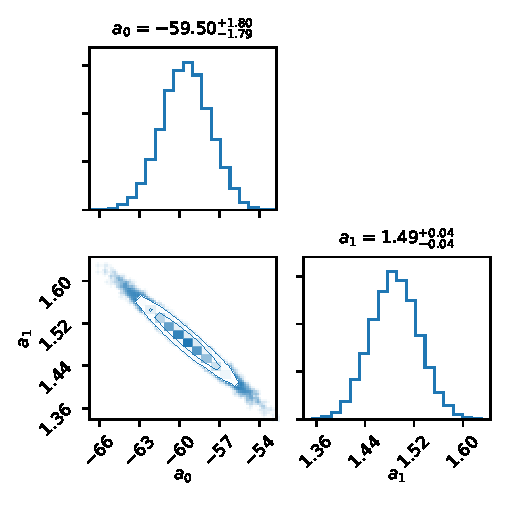
\includegraphics{CodeAndFigures/LinearModelMetropolisHastings.pdf}
    \caption{Joint posterior probability distribution and marginalized posterior probability for the parameters $a_0$ and $a_1$ from the model described in equation \ref{eq:linearModel}}
    \label{fig:LinearHastings}
\end{figure}